\subsection*{Problema 30}
\textbf{Enunciado:} Calcular la integral:
\begin{align*}
\int \dfrac{2x + 1}{3x^3 + 2x - 1} \, dx
\end{align*}

\textbf{Solución:} 
Utilizamos el método de descomposición en fracciones parciales. 
Primero, encontramos las raíces del polinomio denominador:
\begin{align*}
P(x) = 3x^3 + 2x - 1
\end{align*}
Probando con la raíz racional $x = \dfrac{1}{3}$, tenemos:
\begin{align*}
P\left(\dfrac{1}{3}\right) = 3\left(\dfrac{1}{27}\right) + 2\left(\dfrac{1}{3}\right) - 1 = 0
\end{align*}
Por lo tanto, $(3x - 1)$ es un factor del polinomio. Al dividir $P(x)$ entre $(3x - 1)$ mediante división sintética o polinómica, obtenemos el trinomio cuadrático:
\begin{align*}
3x^3 + 2x - 1 = (3x - 1)(x^2 + \dfrac{1}{3}x + 1)
\end{align*}
Para evitar fracciones complejas, multiplicamos y dividimos por $3$ dentro del trinomio:
\begin{align*}
3x^3 + 2x - 1 = (3x - 1)(x^2 + \dfrac{1}{3}x + 1)
\end{align*}

Planteamos la descomposición en fracciones parciales de la forma:
\begin{align*}
\dfrac{2x + 1}{3x^3 + 2x - 1} = \dfrac{A}{3x - 1} + \dfrac{Bx + C}{x^2 + \dfrac{x}{3} + 1}
\end{align*}

Multiplicando ambos lados por el denominador común:
\begin{align*}
2x + 1 = &A\left(x^2 + \dfrac{x}{3} + 1\right) \\
&+ (Bx + C)(3x - 1)
\end{align*}

Evaluando en $x = \dfrac{1}{3}$:
\begin{align*}
2\left(\dfrac{1}{3}\right) + 1 &= A\left(\left(\dfrac{1}{3}\right)^2 + \dfrac{1}{9} + 1\right) \\
\dfrac{5}{3} &= A\left(\dfrac{1}{9} + \dfrac{1}{9} + 1\right) = \dfrac{11}{9}A
\end{align*}
De donde obtenemos $A = \dfrac{15}{11}$.

Igualando coeficientes para las potencias de $x^2$:
\begin{align*}
0 &= A + 3B \implies B = -\dfrac{A}{3} = -\dfrac{5}{11}
\end{align*}

Igualando los términos independientes ($x^0$):
\begin{align*}
1 &= A - C \implies C = A - 1 \\
C &= \dfrac{15}{11} - 1 = \dfrac{4}{11}
\end{align*}

Sustituyendo los valores de $A$, $B$ y $C$ en la integral:
\begin{align*}
\int &\dfrac{2x + 1}{3x^3 + 2x - 1} \, dx = \\
&\int \left( \dfrac{\frac{15}{11}}{3x - 1} + \dfrac{-\frac{5}{11}x + \frac{4}{11}}{x^2 + \frac{x}{3} + 1} \right) dx
\end{align*}

La primera integral es inmediata:
\begin{align*}
\int \dfrac{\frac{15}{11}}{3x - 1} \, dx = \dfrac{5}{11} \ln|3x - 1|
\end{align*}

Para la segunda integral, completamos el binomio en el denominador:
\begin{align*}
x^2 + \dfrac{x}{3} + 1 = \left(x + \dfrac{1}{6}\right)^2 + \dfrac{35}{36}
\end{align*}
Y ajustamos el numerador para que aparezca la derivada del denominador ($2x + \dfrac{1}{3}$):
\begin{align*}
-\dfrac{5}{11}x + \dfrac{4}{11} = -\dfrac{5}{22}\left(2x + \dfrac{1}{3}\right) + \dfrac{55}{132}
\end{align*}

Integrando esta parte obtenemos un término logarítmico y uno de arco tangente:
\begin{align*}
-\dfrac{5}{22} &\ln\left(x^2 + \dfrac{x}{3} + 1\right) \\
&+ \dfrac{9}{2\sqrt{35}} \arctan\left(\dfrac{6x + 1}{\sqrt{35}}\right)
\end{align*}

Combinando todos los resultados, la solución general es:
\begin{align*}
F(x) &= \dfrac{5}{11} \ln|3x - 1| \\
&- \dfrac{5}{22} \ln\left(x^2 + \dfrac{x}{3} + 1\right) \\
&+ \dfrac{9}{2\sqrt{35}} \arctan\left(\dfrac{6x + 1}{\sqrt{35}}\right) + C
\end{align*}

\begin{figure}[H]
	\centering
	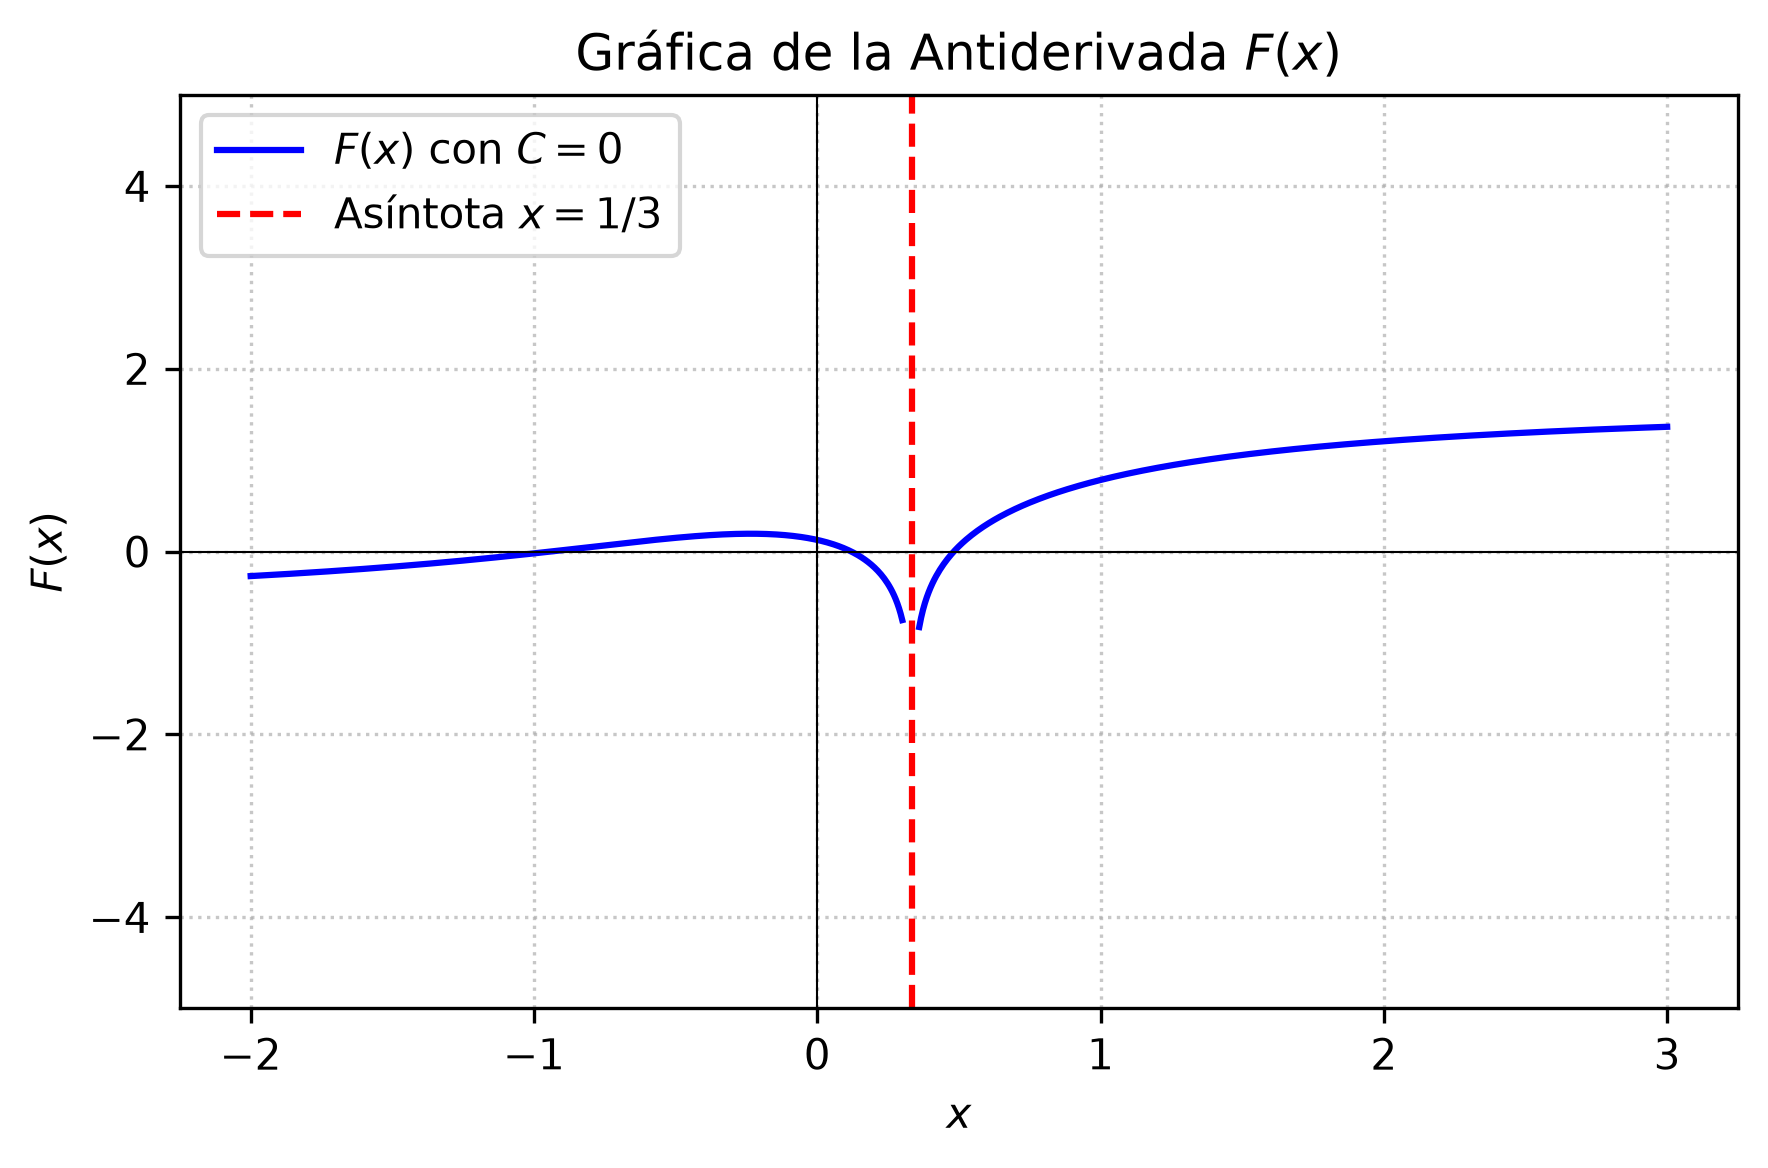
\includegraphics[width=\columnwidth]{semana_03/graficas/SEM03_P30_grafica.png}
	\caption{Representación gráfica de $f(x)$ y su antiderivada $F(x)$ evaluada para la constante de integración $C = 0$ (Problema 30).}
	\label{fig:problema30}
\end{figure}
